\documentclass[20pt,landscape,footrule]{foils}
\paperwidth=1024pt
\paperheight=768pt
\usepackage{color}
\usepackage{geometry}
\usepackage{tabularx}
\usepackage{pause}
\usepackage{hyperref}
\usepackage{pp4link}
% \usepackage{pp4slide}
\usepackage{mpmulti}
\usepackage{graphicx}
% \usepackage{background}
\usepackage{ifthen}
\DeclareGraphicsRule{*}{mps}{*}{}
\usepackage{amsmath, amssymb}   
\geometry{headsep=2ex,hscale=0.9,footskip=10ex} 
\hypersetup{pdftitle={mg},
 pdfsubject={Netgen/NGSolve Quickstart},
  pdfauthor={Joachim Schoeberl},
  pdfkeywords={pdftex, acrobat, ppower4},
  pdfpagemode={FullScreen}
  }

\newcommand\sectionname{}


\begin{document}
% \definecolor{bgblue}{rgb}{0.04,0.39,0.53}
% \vpagecolor{bgblue}


\parindent 0mm\raggedright
\MyLogo{\pauselevel{=1}Joachim Sch\"oberl \hfill 
% \Acrobatmenu{LastPage}{the end} \hfill
% \toplink{workpage}{Jump to Working page} \hfill
\sectionname \hfill
\hfill
Page }


\foilhead{\color{blue}
{\bf A Quick Start with Netgen / NGSolve  } }

Overview
\begin{itemize}
\item \hyperlink{whatisnetgen}{A tour through Netgen/NGSolve}
\item \hyperlink{installing}{How to install Netgen and NGSolve}
\item \hyperlink{runnetgen}{How to use the mesh generator Netgen}
\item \hyperlink{runngsolve}{How to use the Finite Element Solver NGSolve}
\item \hyperlink{programming}{How to program in NGSolve}
\end{itemize}



\foilhead{\color{blue}
{\bf What is Netgen ?  } }
\hypertarget{whatisnetgen}{}
\renewcommand\sectionname{A tour through Netgen/NGSolve}
\begin{itemize}
\item Netgen is an automatic 2D and 3D tetrahedral mesh generator
\item Input can be provided by simple ASCII files (csg - files), or imported from CAD programs via IGES, Step, or STL files
\item Netgen generates essentially unstructured triangular/tetrahedral meshes
\item Netgen comes with a graphical user interface, or can be used as library
\item Netgen is open source based on the LGPL license
\end{itemize}

\foilhead{\color{blue}
{\bf Some Meshes generated by Netgen } }

A machine frame imported via the Step - format, a bunny imported from STL ...

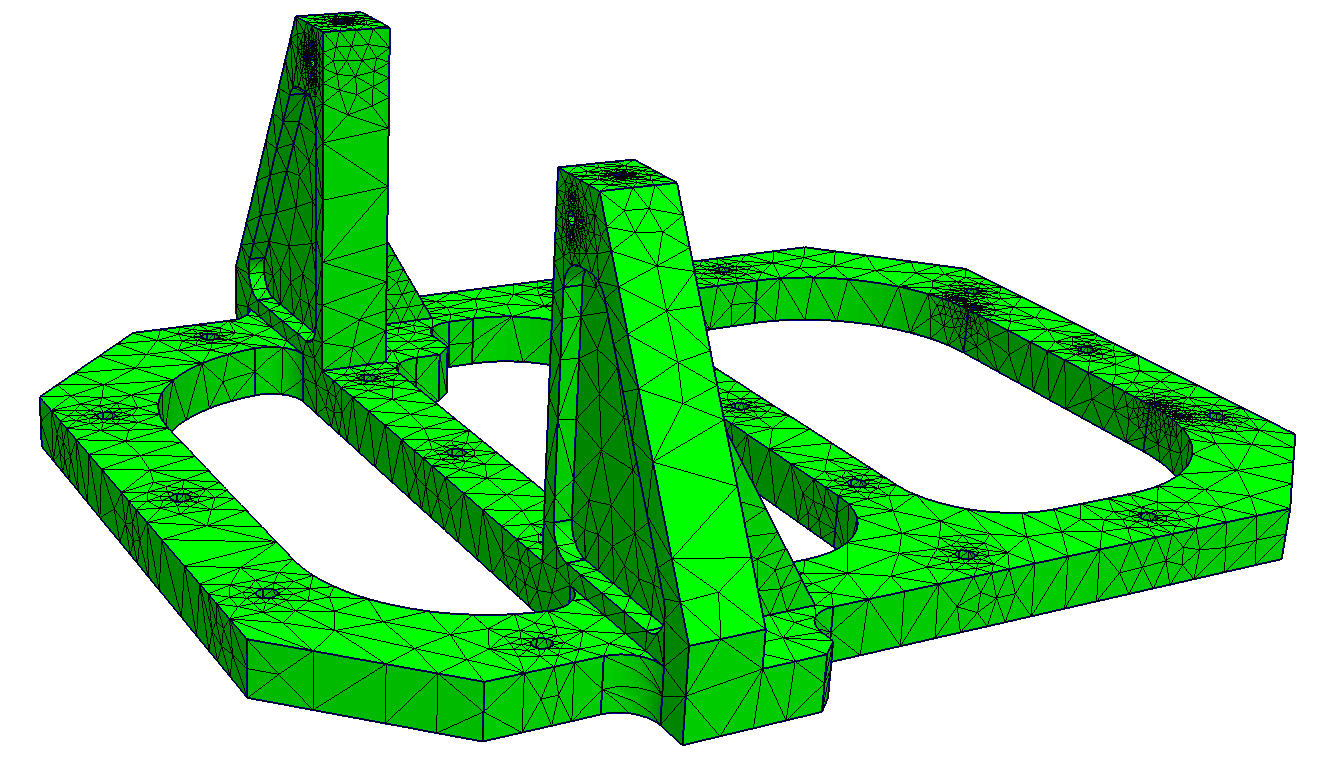
\includegraphics[width=0.5\textwidth]{ng_proe.jpg}
\hspace{0.1\textwidth}
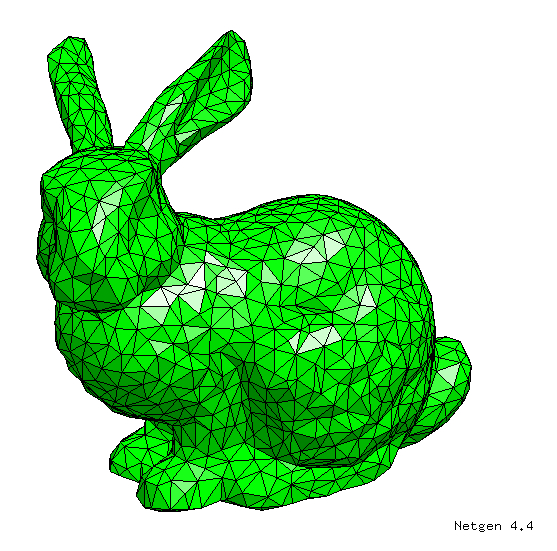
\includegraphics[width=0.3\textwidth]{bunny.jpg}

\foilhead{\color{blue}
{\bf What is NGSolve ? } }
\begin{itemize}
\item NGSolve is a finite element library which can be linked to Netgen
\item contains arbitrary order finite elements of all standard element geometries,
scalar, vector-valued, hybrid DG finite element spaces
\item Integrators for basic equations (heat flow, elasticity, Maxwell, ...)
\item Iterative solvers, a posteriori error estimates, ...
\item There are extension modules for different application areas (ngs-mech, ngs-flow, ...)
\item NGSolve is open source based on the LGPL license
\end{itemize}


\foilhead{\color{blue} Simulation of Mechanical Deformation and Stresses\\}
%
\begin{center}
\begin{minipage}[t]{0.4\textwidth}
Elastic beam: \\
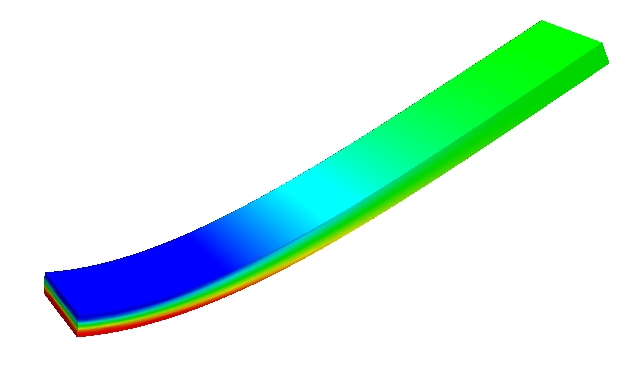
\includegraphics[width=0.7\textwidth]{beam_sol.jpg}
\end{minipage}
\begin{minipage}[t]{0.4\textwidth}
Shell structures: \\
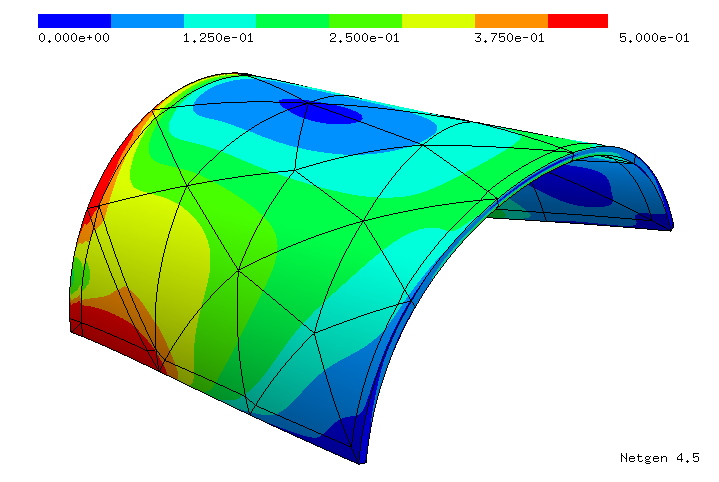
\includegraphics[width=0.7\textwidth]{shell3d.jpg}
\end{minipage}
\end{center}
\vspace{2ex}
\begin{center}
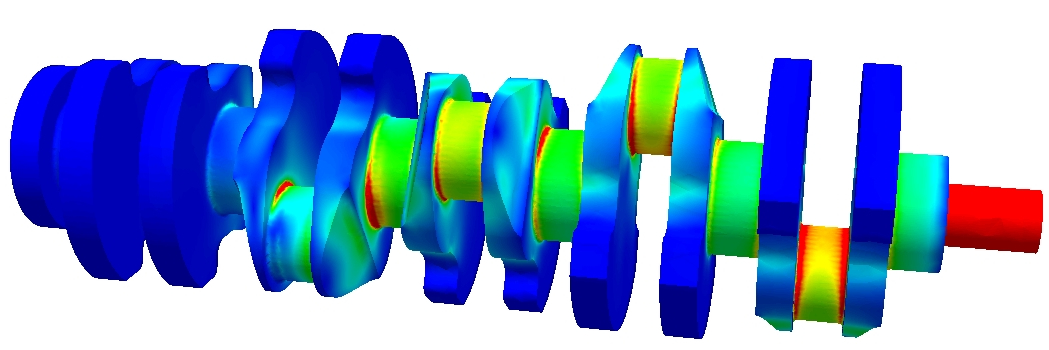
\includegraphics[width=0.6\textwidth]{crankshaft_cut.jpg}
\end{center}


\foilhead{\color{blue} Simulation of Electromagnetic Fields}

\begin{minipage}[t]{0.3\textwidth}
A simple coil: \\[2ex]
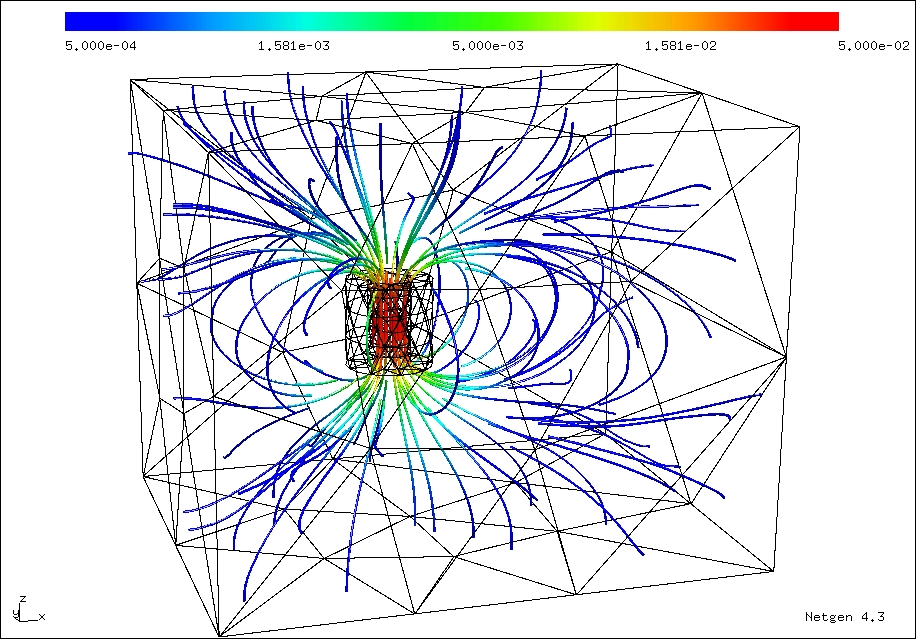
\includegraphics[width=1\textwidth]{d7_fieldlines.jpg} \\[3ex]
Described by \\ Maxwell's equations
\end{minipage} \hspace{0.1\textwidth}
\begin{minipage}[t]{0.58\textwidth}
A transformer built by Siemens - EBG, Linz: \\[2ex]
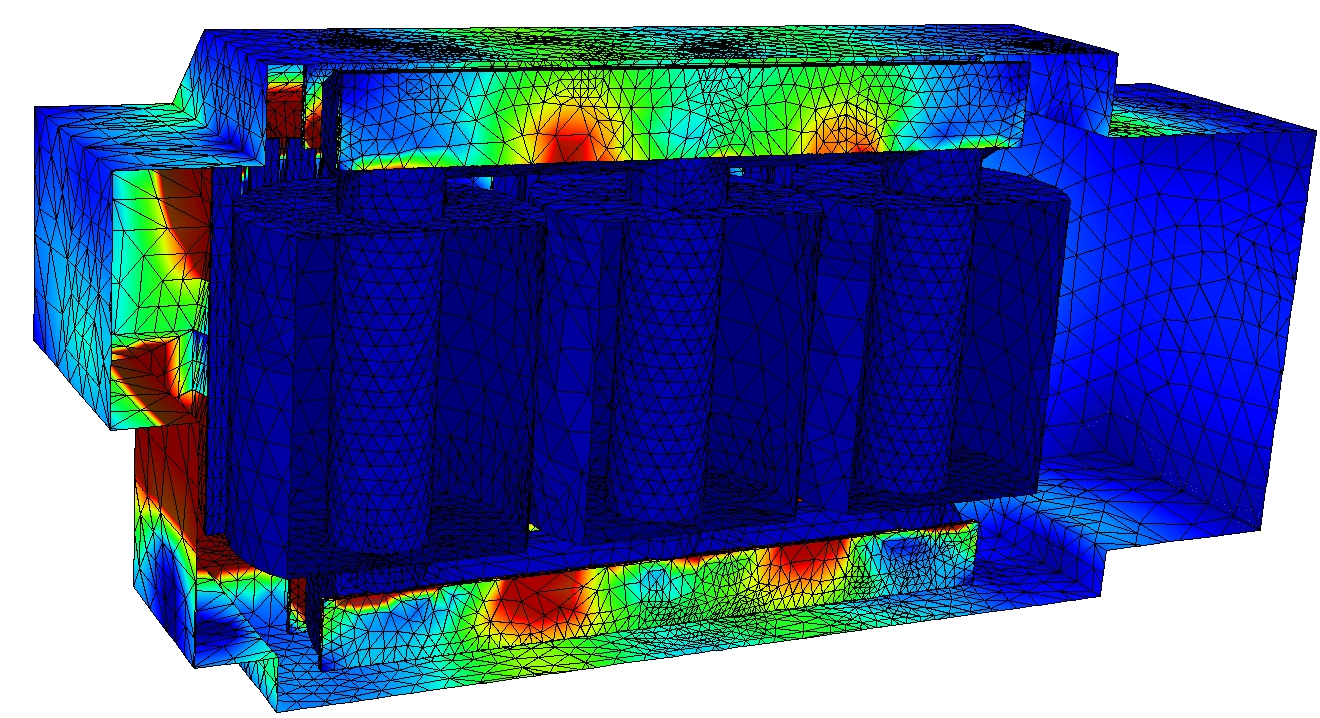
\includegraphics[width=1\textwidth]{TA13037alt_losses_clumps_cut.jpg}
\end{minipage}


\foilhead{\color{blue} Incompressible Flows}

Flow around a disk, Re = 100,  $5^{th}$-order elements: \\[1em]
\begin{minipage}{0.95\textwidth}
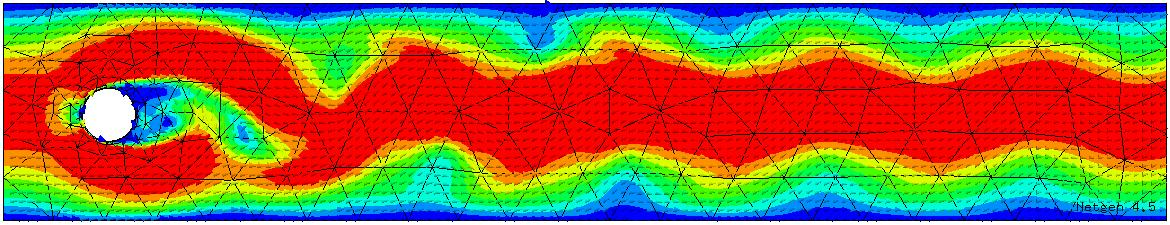
\includegraphics[width=0.8\textwidth]{cylinder_re100.jpg}
\end{minipage}

\vspace{2em}

Flow around a cylinder, Re = 100 \\[0em] 
%
\begin{minipage}{0.95\textwidth}
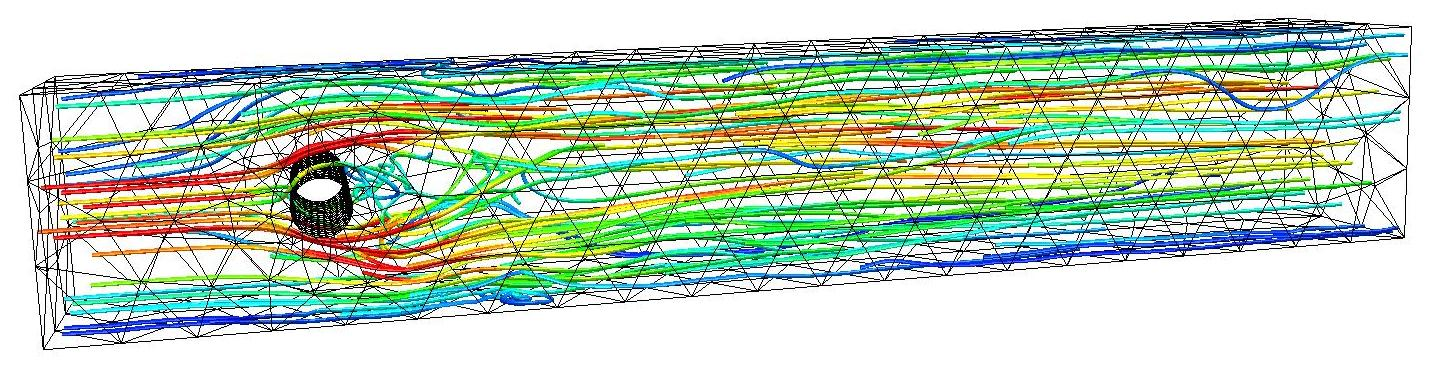
\includegraphics[width=0.8\textwidth]{cylinder3dc.jpg}
\end{minipage}



\foilhead{\color{blue}
{\bf Downloading and Installing Netgen/NGSolve  } }
\hypertarget{installing}{}
\renewcommand\sectionname{Installing Netgen/NGSolve}
The codes and most detailed informations are available from sourceforge:

\begin{itemize}
\item http://sourceforge.net/projects/netgen-mesher/
\item http://sourceforge.net/projects/ngsolve/
\end{itemize}

There are source packages, binary packages (windows), and the latest code in SVN

Latest installation information is on the Wiki - pages
\begin{itemize}
\item http://netgen-mesher.wiki.sourceforge.net
\item http://sourceforge.net/apps/mediawiki/ngsolve
\end{itemize}

\foilhead{\color{blue}
{\bf Installing Netgen/NGSolve on Windows} }

There are 3 different options:
\begin{itemize}
\item Install Netgen/NGSolve executables from the installer. 
This is enough to run Netgen/NGSolve.

\item Compile Netgen and NGSolve yourself using 
Microsoft Visual C++ (free express edition is enough). This requires a couple of
additional libraries such as Tcl/Tk/Tix/Togl, pthread-win32 for
Netgen, and Lapack for NGSolve.  You can work on the whole code.

\item Install Netgen binary, and compile NGSolve yourselves. 
This only requires the Lapack library. This version is recommended if
you want to implement some finite element stuff. It generates the
dynamic link library ngsolve.dll, which must be copied into the Netgen directory.
\end{itemize}


\foilhead{\color{blue}
{\bf Installing Netgen/NGSolve on Linux/Unix/Mac} \\}
%
\begin{enumerate}
\item Install 3rt party libraries as described in the installation manual on wiki (tcl-devel, tk-devel, tix, togl1.7, glut)
\item Compile and install Netgen:
\begin{verbatim}
> ./configure --prefix=/opt/netgen
> make install
\end{verbatim}
It puts the executable, tutorials, and header files into the installation directory.

\item Compile and install NGSolve. It requires some header files from Netgen
\begin{verbatim}
> ./configure --prefix=/opt/netgen --with-netgen=/opt/netgen
> make install
\end{verbatim}
It puts the shared library libngsolve.so into the installation directory.
\end{enumerate}
Add the /opt/netgen/bin to your PATH, and /opt/netgen/lib to your LD\_LIBRARY\_PATH variable.

\foilhead{\color{blue}
{\bf Running the Mesh Generator Netgen } \\}
%
\hypertarget{runnetgen}{}
\renewcommand\sectionname{Running Netgen}
Start the program 'netgen'. Select ``File $\rightarrow$ Load Geometry'', and load, e.g., the file {\em /opt/netgen/share/netgen/boxcyl.geo}. The window should look like this:

\begin{center}
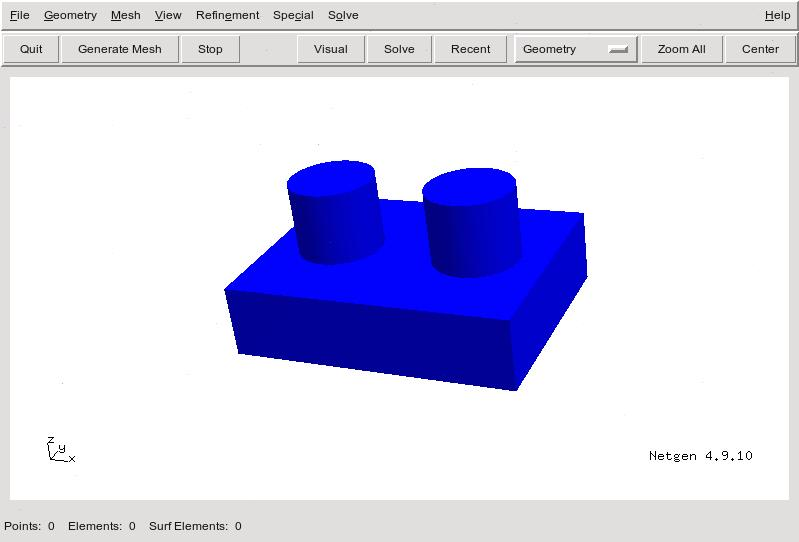
\includegraphics[width=0.4\textwidth]{netgen-geometry.jpg} \\[2ex]
\end{center}

Moving the mouse keeping the left button, the middle button, or right button pressed rotates, moves, or zooms the model.

\foilhead{\color{blue}
{\bf Generating the Mesh } \\}
%
Push the button ``Generate Mesh'' to generate a mesh:
\begin{center}
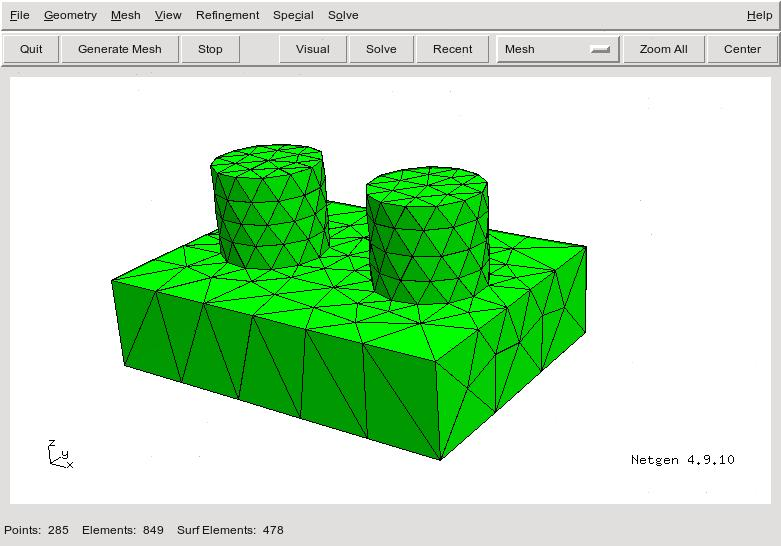
\includegraphics[width=0.4\textwidth]{netgen-mesh.jpg} 
\hspace{0.1\textwidth}
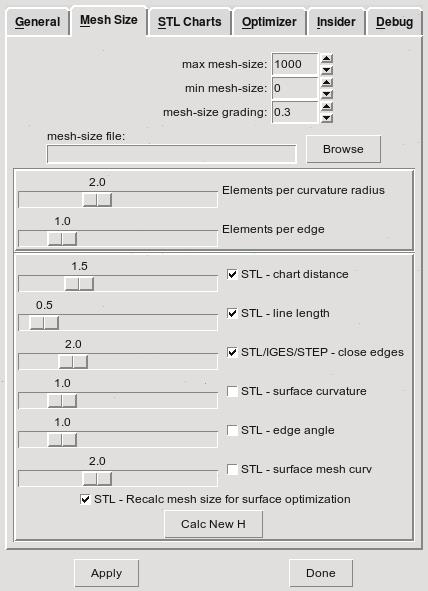
\includegraphics[width=0.25\textwidth]{meshingoptions.jpg} 
\end{center}
With ``Mesh $\rightarrow$ Meshing Options'' you can set parameters. E. g., a general Mesh granularity from 'very fine' to 'very coarse', or a maximal mesh size.

\foilhead{\color{blue}
{\bf Define the geometry} \\}
Supported Geometry formats are
\begin{itemize}
\item 2D geometries (the .in2d files)
\item 3D constructive solid geometries (the .csg files)
\item surface triangulations (.stl files)
\item IGES and Step files, (requires the optional OpenCascade geometry kernel)
\end{itemize}

\foilhead{\color{blue}
{\bf The 3D CSG - Files} \\ }
You specify the the geometry in an ASCII file. Example:

\begin{verbatim}
algebraic3d
solid cube = orthobrick (0, 0, 0; 1, 1, 1);
solid cyl = cylinder (0.5, 0.5, 0; 0.5, 0.5, 1; 0.03);
solid main = cube and not cyl;
tlo main;
\end{verbatim}
One defines a solid 'cube', an infinite cylinder solid 'cyl', and forms the intersection of the cube and the complement of the cylinder. The Top-Level-Object (tlo) 'main' is going to be meshed. Several tlo will lead to several regions (sub-domains). 

\begin{itemize}
\item The syntax is described in the Netgen user manual
\item Have a look into the various .geo examples
\end{itemize}


\foilhead{\color{blue}
{\bf The 2D Files} \\[-1em] }
You specify the geometry by a set of curves. This gives a square:
\begin{verbatim}
splinecurves2dv2
2
points
1       0       0     -maxh=0.01
2       1       0
3       1       1
4       0       1
segments
1       0       2       1       2       -bc=1  -maxh=0.1
1       0       2       2       3       -bc=1
1       0       2       3       4       -bc=1
1       0       2       4       1       -bc=2
materials
1       domain1   -maxh=0.3
\end{verbatim}
\newpage

{\em splinecurves2dv2} is the keyword for the 2D inputs, version 2. 

Next comes a global grading parameter.

The points given with index and coordinates

The curves are given by the sub-domain number on the left, sub-domain number on the right, number of points to define the curve, and the point indices. sub-domain number 0 means exteriori (which is not meshed). A straight line is defined by 2 points, a second order spline by 3. 

The flag '-maxh' sets the  maximal element diameter  at a point, along a curve, or in a region (material).

The flag '-bc' defines the boundary condition index.

\begin{itemize}
\item Have a look into the various .in2d examples
\end{itemize}

\foilhead{\color{blue}
{\bf Running NGSolve} \\ }
\hypertarget{runngsolve}{}
\renewcommand\sectionname{Running NGSolve}

When NGSolve is installed, you find a 'Solve' pull down menu item. 

Select 'Solve $\rightarrow$ Load PDE', and load, e.g. the file {\em /opt/netgen/share/ngsolve/d4\_cube.pde}. Just a Poisson equation.

Push the solve button. Watch the shell window for the ongoing actions.

Push the Visual button for setting the visualization. Switch 'Scalar
Function' to 'u'. Activate a clipping plane, and set 'Clipping Plane
Sol.' to 'Scalar Function'.

Restart, and load example 'd5\_beam.pde'. It is a mechanical deformation problem. Solve. Set 'Vector function' to 'u'. Click deformation, and set 'scale' to 100. Choose a 'Scalar function'.

Restart, and load example 'd7\_coil.pde'. It is a Maxwell problem (magnetostatics). Solve. Switch on a clipping plane. Select a Vector-Function 'flux'. Choose 'Clipping Plane Sol' to be 'Vector Function'. BUG: switch off Use Texture.


\foilhead{\color{blue}
{\bf NGSolve script file for Poisson example} \\[-2em]}
%
$$
\mbox{Find } u \in H^1 \mbox{ s.t. } \qquad 
\int_\Omega \lambda \, \nabla u \cdot \nabla v \, dx + \int_{\partial \Omega} \alpha u v \, ds
= \int_\Omega f v \, dx \qquad \forall \, v \in H^1
$$
% \\[3em]
{
\small
\begin{verbatim}

define coefficient lam      1,
define coefficient alpha    1e5, 1e5, 1e5, 0, 
define coefficient cf       sin(x)*y,

define fespace v -h1 -order=4
define gridfunction u -fespace=v 

define bilinearform a -fespace=v -symmetric
laplace lam
robin alpha

define linearform f -fespace=v
source cf

define preconditioner c -type=multigrid -bilinearform=a -smoothingsteps=1 -smoother=block

numproc bvp np1 -bilinearform=a -linearform=f -gridfunction=u -preconditioner=c -prec=1e-8
\end{verbatim}
}


\foilhead{\color{blue} Interplay of Netgen and NGSolve}
\hypertarget{programming}{}
\renewcommand\sectionname{NGSolve Programming}

\begin{center}
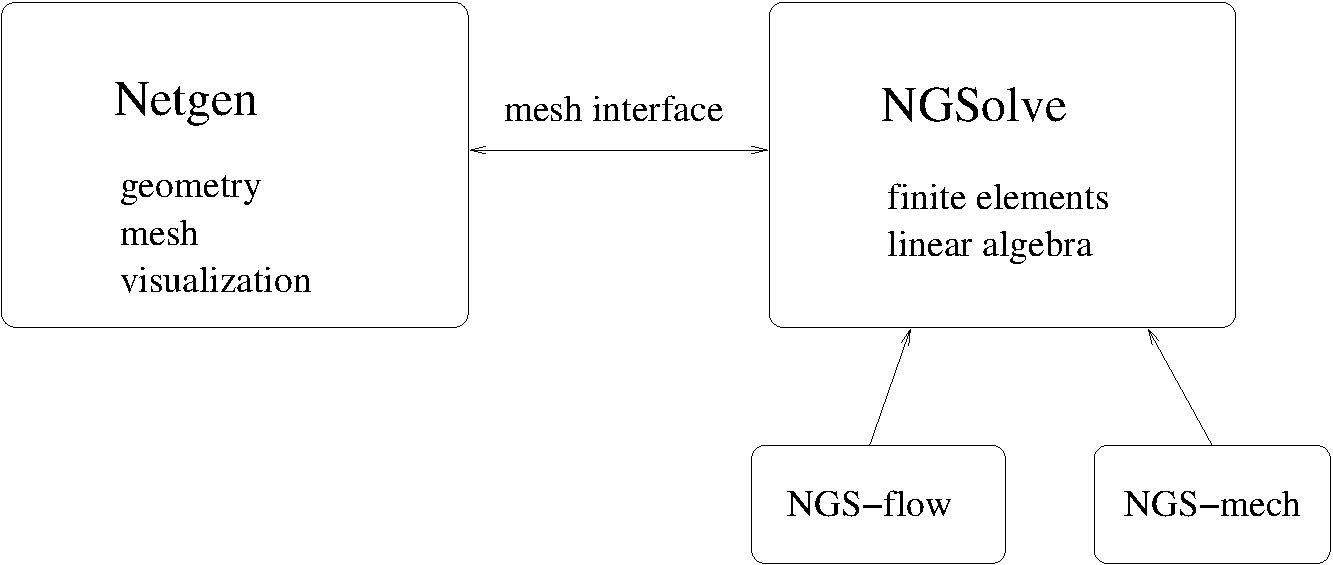
\includegraphics[width=0.6\textwidth]{interplay.pdf} 
\end{center}

\begin{itemize}
\item Netgen knows the geometry, and maintains the mesh, does visualization
\item NGSolve does the finite elements and linear algebra
\item Connection is via the mesh interface (NGSolve: {\em class MeshAccess})
\end{itemize}

Application classes can be loaded as shared libraries into NGSolve


\foilhead{\color{blue} The layers of NGSolve }

\begin{center}
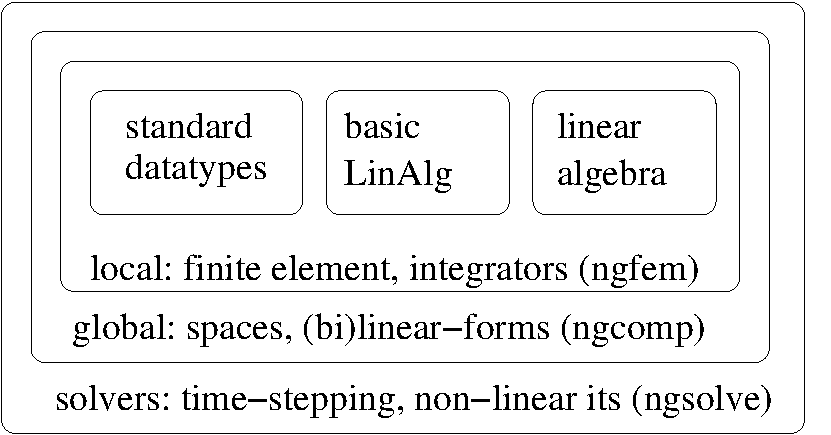
\includegraphics[width=0.6\textwidth]{layers.pdf} 
\end{center}

\vspace{2em}

The layers correspond to namespaces (and sub-directories)


\foilhead{\color{blue} Central NGSolve \bf classes \\}
%
\begin{itemize}
\item FiniteElement (ngfem): \newline
  Provides shape functions and derivatives on reference element
\item ElementTransformation (ngfem): \newline
  Represents mapping to physical elements, computes Jacobian
\item Integrator (ngfem): \newline
  Computes element matrices and vectors 
\item FESpace (ngcomp): \newline
  Provides global dofs, multigrid-transfers and smoothing blocks
\item BilinearForm/LinearForm (ngcomp): \newline
  Maintains definition of forms, provides matrix and vectors
\item PDE (ngsolve): \newline
  Container to stores all components
\end{itemize}



\foilhead{\color{blue} Where to start programming ?}

The directory 'my\_little\_ngsolve' provides a play ground to start
NGSolve programming.  

Run 'make intall' in the directory 'my\_little\_ngsolve'. It will generate and install a shared library with the new stuff.

\begin{enumerate}
\item
Have a look into 'myElement.hpp' (.cpp), 'myFESpace.hpp' (.cpp), 'myIntegrator.hpp' (.cpp). Explains how to implement elements, finite element spaces, and integrators

{\bf Exercise:} Start adding elements (quadrilateral, tetrahedral element), and integrators (Neumann b.c.)

\item
Have a look into 'demo\_instat.cpp'. It demonstrates how to write a simpe solver for parabolic equations. Works with linear algebra objects

{\bf Exercise:} Implement the Newmark solver for second order hyperbolic equations.

\item
Have a look into 'demo\_coupling.cpp'. It demonstrates how to work with finite elements, how to mange dofs, and the elementtransformation.
\end{enumerate}

More prgramming demos are in 'programming\_demos'. These show how to write stand-alone programs using the NGSolve objects.








\end{document}


